\documentclass[border=8pt]{standalone}
\usepackage{tikz}
\usetikzlibrary{arrows.meta,positioning,calc}
\begin{document}
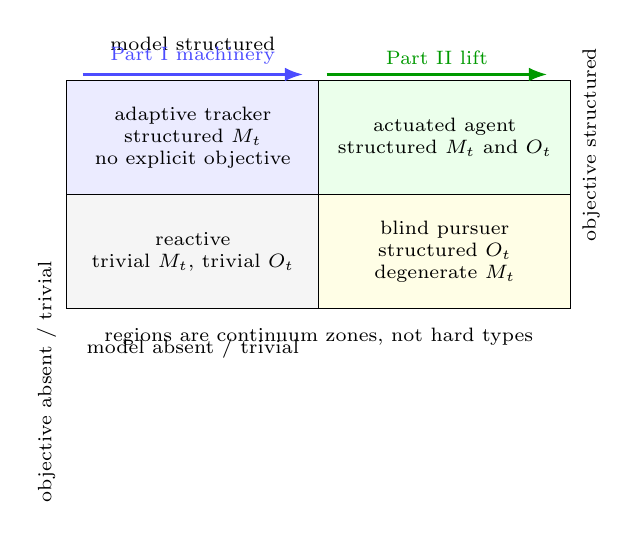
\begin{tikzpicture}[
  cell/.style={draw, align=center, minimum width=3.2cm, minimum height=1.45cm, font=\scriptsize},
  label/.style={align=center, font=\scriptsize},
  arr/.style={-Latex, thick}
]

\node[cell, fill=gray!8] (react) at (0,0) {reactive\\trivial $M_t$, trivial $O_t$};
\node[cell, fill=yellow!10] (blind) at (3.2,0) {blind pursuer\\structured $O_t$\\degenerate $M_t$};
\node[cell, fill=blue!8] (tracker) at (0,1.45) {adaptive tracker\\structured $M_t$\\no explicit objective};
\node[cell, fill=green!8] (act) at (3.2,1.45) {actuated agent\\structured $M_t$ and $O_t$};

\node[label, above=0.25cm of tracker] {model structured};
\node[label, below=0.25cm of react] {model absent / trivial};
\node[label, left=0.25cm of react, rotate=90] {objective absent / trivial};
\node[label, right=0.25cm of blind, rotate=90] {objective structured};

\draw[arr, blue!70] (-1.4,2.25) -- node[above, font=\scriptsize] {Part I machinery} (1.4,2.25);
\draw[arr, green!60!black] (1.7,2.25) -- node[above, font=\scriptsize] {Part II lift} (4.5,2.25);

\node[label, below=0.85cm of $(react)!0.5!(blind)$] {regions are continuum zones, not hard types};

\end{tikzpicture}
\end{document}
